\begin{minipage}{.6\linewidth}
	\vspace{-3cm}
	\item O sistema consiste de dois blocos, $A$ e $B$, de 30 e \SI{10}{\kilogram}, respectivamente, e das polias de \SI{2.5}{\kilogram} $C$ e $D$, que podem ser tratadas como dois discos finos. Determine a velocidade do bloco $A$ após o bloco $B$
	haver se elevado \SI{1.5}{\meter}, partindo do repouso. Suponha que a corda não desliza nas roldanas e despreze
	a massa da corda.
\end{minipage}
\begin{minipage}{.4\linewidth}
	\begin{flushright}
		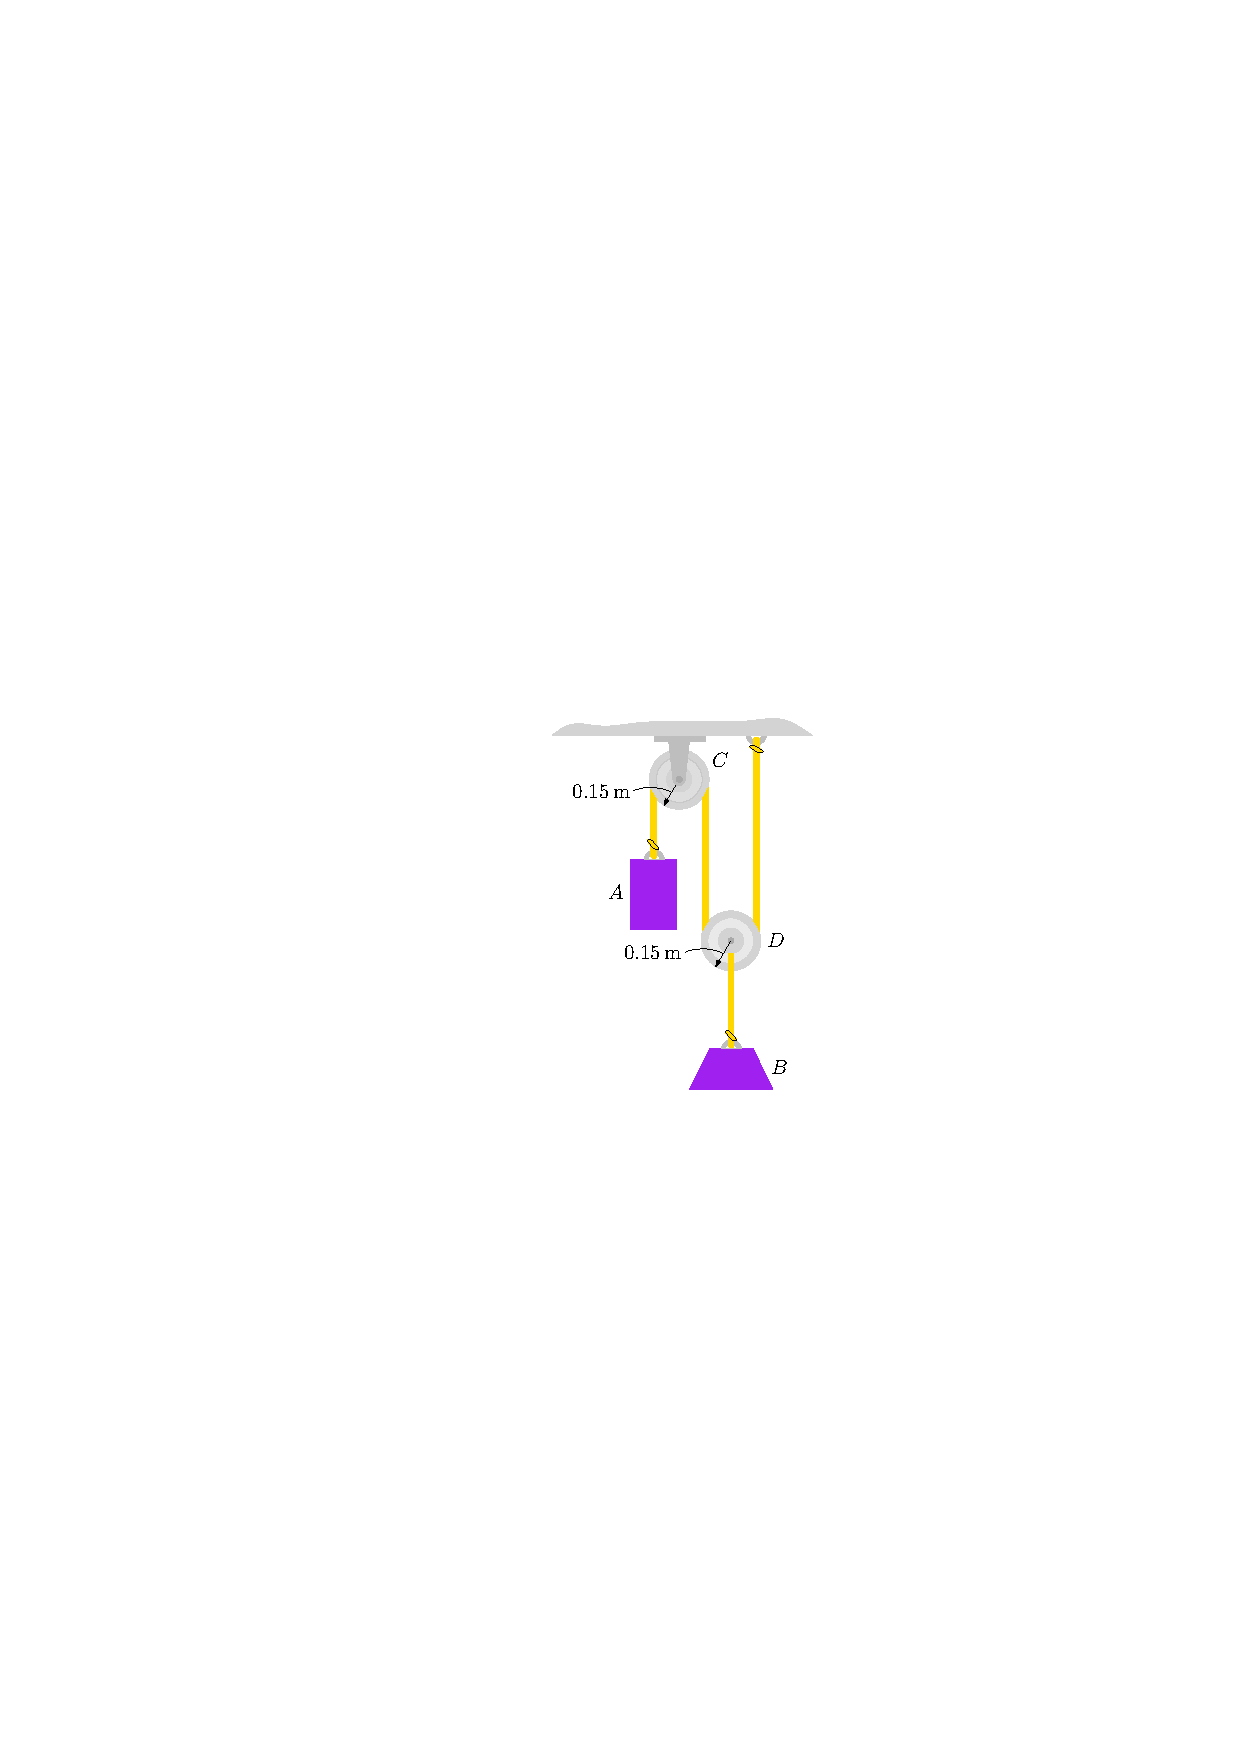
\includegraphics[scale=1.2]{../../images/draw_5}
	\end{flushright}
\end{minipage}